\documentclass[11pt]{article}
\usepackage[margin=1in]{geometry}
\usepackage{amsmath}
\usepackage{amssymb}
\usepackage{booktabs}
\usepackage{longtable}
\usepackage[T1]{fontenc}
\usepackage{graphicx}
\usepackage[hidelinks]{hyperref}
\usepackage{microtype}
% float placement: let figures sit near their reference and keep floats from queueing to the end
\renewcommand{\topfraction}{0.9}
\renewcommand{\bottomfraction}{0.9}
\renewcommand{\textfraction}{0.05}
\renewcommand{\floatpagefraction}{0.7}
\setcounter{topnumber}{3}
\setcounter{totalnumber}{4}
\graphicspath{{figures/}}

\title{How much do LLM agents actually couple?\\
Tabulated policies and a mean-field criterion for the exposure, memory\\
and format knobs of small open-weight agents}
\author{Luigi Simeone\\ \small Independent researcher}
\date{October 2026}

\begin{document}
\maketitle

\begin{abstract}
Populations of language-model agents show collective behaviour that single agents do not; recent work describes it with spin models in which agents
are coupled, feel an intrinsic field and order above a threshold. We ask the
engineering question instead: given the knobs set when such a system is built, how strong is the coupling, and where do they keep a population below threshold? On two small open-weight models (Qwen3, 0.6 and 1.7 billion parameters), in an abstract two-label game, we tabulate the policy of an agent
from its logits for every configuration of its peers and fit a spin model to
the table. Three knobs are varied on a paired design of ten formulations: the number of peers shown (2 to 30), the memory of the agent's
own past states (0 to 3) and the format of the peer list; every hypothesis and rule was written before the data. The coupling per peer falls as more
peers are shown, in both models, and from 7 peers on the larger model responds
to the fraction of peers that agree, not to their number. Memory of one's own states reduces the coupling to the peers and adds persistence. The list separator does not move the coupling; presenting the peers as a count rather than a list lowers it in the larger model. The criterion for the instability of
the disordered state is the slope of the mean-field map on the tabulated
policy, with a combinatorial ceiling set by the number of peers sampled; the linear summary of earlier work overestimates order, and we decompose the gap exactly. From 4 peers on, the 0.6B model sits below threshold in nine of
ten formulations, not for lack of interaction, which alone is at or above threshold in six of them, but because the label bias flattens its response to the peers, while the 1.7B model sits above it in most
formulations. The prompt formulation shifts the coupling by an order of
magnitude, so every coupling is reported with its formulations.
\end{abstract}

\section{Introduction}

Work on the collective behaviour of language-model agents has so far set out to explain emergence. Okawa~\cite{okawa2026} builds a spin model of multi-agent debate
with an analytic threshold; De Nobili~\cite{denobili2026} fits an
interaction and a field to the update logs of agents on a lattice and finds
a regime dominated by the intrinsic field; El et al.~\cite{el2026} fit an
Ising model on a signed network to communities of agents; De Marzo et
al.~\cite{demarzo2026} show hysteresis and tipping points under stubborn
agents with a mean-field spinodal; Flint et al.~\cite{flint2026}
precompute the policy of an agent from its logits for every memory state
and simulate at zero cost. Each of these papers takes the collective order as the thing to be explained.

In applications where governance and auditability are requirements,
collective order is instead a risk that has to be contained, and the question becomes in
which region of the design parameters a population of agents stays free of
collective behaviour not reducible to its components. The knobs that practitioners set (how many peers an agent reads, in what form, and how much of its own history it keeps) correspond to physical quantities, namely a coupling between agents and a range of the coupling in time. Feedback by itself does not produce collective order: a thermostat is a loop and shows no emergence. Collective order appears when the update map amplifies a small imbalance, that is, when the gain of the loop is large. This paper measures the first of these quantities, the coupling to the peers, and gives a criterion for which side of the threshold a population sits on.

What is new here, as far as we know, is the following. The coupling is measured as a joint function of exposure, memory and format in a population of agents, with one method (policies tabulated from the logits), on a paired design of formulations, and with a mean-field criterion that is checked against the dynamics. We also report a descriptive regularity in the shape of the response across the formulations of a model, together with the null models that reproduce it. The signs of the
single-shot effects are already known and we do not claim them: conformity grows with the
number of peers~\cite{bellina2026}, with the history of the
peers~\cite{weng2025,ashery2025} and with reasons above a bare
list~\cite{cho2025}. Nor is the measurement battery new. Hysteresis under stubborn agents comes from~\cite{demarzo2026}, the tabulation from the
logits from~\cite{flint2026}, and the reading of the opinion from the logits from~\cite{brockers2026}; we adapt these methods, as stated where each is used, and cite them.

Terminology. Subcritical means, in the sense of branching processes, an
effective gain below one: the field-dominated regime. It is the
``indifferent'' phase of~\cite{el2026} and the ``field-dominated
crossover'' of~\cite{denobili2026}; their ordered phase below the social
critical point is our supercritical regime; the ``subcritical'' amplification
of~\cite{liu2026} on feed-forward trees is a different transition. We do
not claim complexity in the strong sense: the collectives measured here are
described by mean-field models. For a labelled population three classes
are read from the fixed points of the mean-field map of its own sector:
spontaneous order when the map has two stable fixed points (bistability,
with two branches and hysteresis); field-dominated consensus when it has
one stable fixed point at $|m|$ close to 1, the population agreeing on the
label the bias favours; disorder when the map has a single stable fixed
point with $|m^*|$ at or below 0.9, a partial agreement that does not reach
unanimity. The classes ordered and disordered of $F'(0)$ refer to the symmetrised map; they say whether the disordered point is unstable, and they say nothing about whether the labelled population reaches consensus.

\section{Related work}

\paragraph{Spin models of agent populations.} Okawa~\cite{okawa2026} models
debate as Boltzmann updates on a local energy, with a field split into a
task-aligned part and a bias part and a conformity parameter per agent.
De Nobili~\cite{denobili2026} fits $\text{logit}\,P(s'=+1\mid k) =
2(h + Jk)$, with $k$ the sum of four neighbours, to update logs, and finds
$J$ at most about 0.35 for llama against $h$ about 2.8, values of a fit
weighted by the inverse decoding scale and read at the low end of that
scan; the ratio $h/J$ is proposed as a diagnostic of the reliability of a
consensus. El et
al.~\cite{el2026} fit five couplings on communities of 32 agents with
free-text messages and find them in the ordered phase, with the critical
point from the peak of the susceptibility of the fitted model. De Marzo et
al.~\cite{demarzo2026} fit $P(m) = \tfrac12\{\tanh[\beta(m+h)]+1\}$ on 50
agents, find $\beta>1$ for most models and derive the spinodal and the
tipping point under stubborn agents. Flint et al.~\cite{flint2026} study
group-size effects in the naming game with policies precomputed from the
logits, validated against open generation for their game and models; Ashery et al.~\cite{ashery2025}
show emergent conventions and collective bias. Tanaka~\cite{tanaka2026} explains symmetry breaking in neutral naming games as sampling noise amplified at finite size; De Nobili and co-authors~\cite{denobiling2026} study the microscopic dynamics of consensus formation in naming games. Riedl~\cite{riedl2026} tests dynamic emergence
with a partial information decomposition.

\paragraph{Single-shot conformity.} Bellina, De Marzo and
Garcia~\cite{bellina2026} read the probability of the wrong answer from
the logits against 0 to 10 confederates; Weng, Chen and
Wang~\cite{weng2025} measure conformity against the majority size and the
rounds of history; Cho, Guntuku and Ungar~\cite{cho2025} measure herding
under five presentation formats and order effects. None fits a spin model
or runs a population.

\section{Setup}

\paragraph{Game, models, formulations.} Each agent holds one of two labels,
A or B; at each update it reads the states of some peers and outputs its
own. The prompt is in the third person, the answer is forced to a JSON
object with one key, and the state is read from the logits of the two
label tokens after the imposed JSON prefix: no text is generated. The
quantity tabulated is a first-token policy, the conditional of the next
token after the prefix with the thinking mode disabled and no system
prompt; the mass on the two label tokens is 0.9997 on average on the
0.6B (minimum 0.9663), 1.0000 on the 1.7B and 0.9815 on SmolLM2
(minimum 0.7955). A sampled control declared after the main analysis (two
wordings, 4 peers, all 16 configurations, 100 free samples each at scale 0.7
without the prefix) finds the first-token policy representative on the
1.7B (0.1\% unparseable, mean absolute difference 0.007, same side of
one half in 32/32 pairs); on the 0.6B the answers in JSON form agree in the
same way (0.058, 31/32) but 26.9\% of the answers are prose without
a JSON object within 12 tokens (53.8\% in one wording), 18.1\% within 40, a limitation of the tabulation on the small model. The validation of~\cite{flint2026}
concerns their game and models. The five original wordings are five paraphrases of one structure (Appendix~A): third
person, labels always named as A then B, the number and the list of peers,
an optional memory sentence, the JSON instruction at the end. The label tokens, their order, the person, the position of the instruction, a system prompt, and a decisional against a descriptive instruction are not varied. Every count ``in $n$ formulations of ten'' below is a
frequency inside this family. At $k=0$ the prompt contains nothing about
the agent itself, the convention of~\cite{demarzo2026}; every class and
count of Table~\ref{tab:exposure} is at $k=0$. The models are
Qwen3-0.6B in float32 and Qwen3-1.7B in bfloat16 on a laptop CPU; a second
family, SmolLM2-1.7B-Instruct, is used in one result and in one limitation. Ten
formulations of the prompt are shared by every cell: five wordings in two
list formats (comma, lines); for the exposure and format results the five
wordings were also rendered in two further formats (semicolon, brackets),
for twenty. Every effect of a knob is a paired difference inside a
formulation. The wording is the independent unit: every interval on a
paired difference that supports a finding is a $t$ interval on the
per-wording means, while the intervals of the precision checks and of the
controls remain percentile bootstraps over the formulations (a percentile
bootstrap over five wordings, used in a first version, covers 0.824 to
0.846 in a simulation with the variances of these data and was
replaced). After the analysis of the first five, five new wordings with a different structure
(first person, B named before A, instruction first; Appendix~A) were
tabulated at 2, 4 and 7 peers and at 4 peers with memory 3 on both
models, with the rule declared before the data: the exposure and memory
findings are judged on the ten wordings, and the five new alone are the
out-of-family replication.
The game has no ground truth, so only order is measured here; accuracy is a separate quantity and will be measured in the next phase.

\paragraph{Knobs.} In the list channel the agent sees the ordered list of
the states of $e$ peers ($e$ is the exposure); in the count channel, used as
an internal replication, only how many hold each label. Exposure is 2, 4,
7 in the grid of 8 agents on the complete graph and 2 to 30 in the
tabulation of the response with 32 agents. Memory of length $k$ adds a
sentence with the agent's own last $k$ states; $k$ is 0 or 3 in the grid
and 0 to 3 in the memory curve.

\paragraph{Tabulated policies.} Following~\cite{flint2026}, the gap between
the two label logits is read once for every configuration of the peers
and of the memory, and the population dynamics runs in numpy at zero model
cost. The flipped sector, with the label roles swapped, is the same text as
the unflipped sector with the peer states negated, so its gap follows by
identity; the label bias is fitted inside a sector and the interaction
from the odd part of the table. The grid dynamics runs each sector with its
own biased table and averages the measures over the two sectors (the
global-flip protocol); the mean-field map and the consistency check at 200
agents use the symmetrised table, and the classes of the labelled
population use the table of sector A. Up to 4 peers every ordering of the list is enumerated;
from 7 on, 8 orderings per sum are tabulated in the grid and 32 in the
cells at 7, 10 and 30 peers, and the effect of the sampling is measured.
Every memory tuple is enumerated, so the fitted quantities do not depend on
how the dynamics initialises the memory.

\paragraph{Estimators.} The coupling per peer $\tilde J$ is the slope over
two of the regression of the mean gap on the sum $k$ of the peer states;
the total push is $\bar z\tilde J = e\tilde J$; the label bias $\tilde h$
is the intercept over two inside a sector, so that the fitted gap is $\operatorname{logit} P(+\mid k) = 2(\tilde h + \tilde J k)$ and the bias expressed in logit is $2\tilde h$; it is positive (toward A, the label named
first in the five original wordings) in 10/10 formulations on the 0.6B and in 8 to 9 of 10
on the 1.7B, and, in a cell with the labels named as B then A, falling to 0.34 and 0.09 (paired $-$0.47 $[-1.04, 0.10]$ and $-$1.97 $[-3.04, -0.90]$, t intervals on the five per-wording means, the first including zero): on these five wordings the order of mention is 58\% and 96\% of the bias, and on the 1.7B it moves $\tilde J$ too ($-$0.55 $[-0.82, -0.27]$). The share does not transfer to the five new wordings, three of which name B first and keep a bias toward A: with the naming order swapped inside each new wording (a cell declared after the ten-wording analysis, 4 peers, no memory, both models; t intervals on the five per-wording means) $\tilde h(\text{A first}) - \tilde h(\text{B first})$ is $-$0.61 $[-2.04, 0.81]$ on the 0.6B (positive in 2/5 wordings) and 0.96 $[-0.41, 2.33]$ on the 1.7B (4/5, 39\% of the A-first mean), and the bias stays toward A in 10/10 formulations of each model when B is named first. Over the ten wordings the order moves the bias on the 1.7B (1.47 $[0.70, 2.24]$, positive in 9/10 wordings, 65\% of the A-first mean as a point estimate, toward A in 16/20 formulations when B is named first) and not on the 0.6B ($-$0.07 $[-0.79, 0.64]$, toward A in 20/20). So on the small model the order effect has no consistent sign across the two wording structures (positive in 5/5 of the original wordings and in 2/5 of the new ones) and is not detected over the ten wordings, with a half-width equal to the bias itself, while the bias toward A persists in 20/20 formulations when B is named first; on the large model the point estimate puts about two thirds of the bias on the order of mention (from a third to nearly all of it within its interval), and alternating the order reduces it there but does not remove it on the small model. A cell with the label tokens X and Y in place of A and B (X the + label, the same ten wordings in both naming orders, 4 peers, no memory, declared before the data) separates the token from the order: on the 0.6B the bias toward X is present in both orders (mean over the two orders 0.64 $[0.42, 0.86]$ over ten wordings, toward X in 18/20 and 16/20 formulations) with a difference between orders that is not detected ($-$0.20 $[-1.19, 0.79]$, a half-width larger than the bias), a preference for one token of the pair of the size of the one for A (0.69 over the two orders on A/B); on the 1.7B no token is preferred (mean over the two orders $-$0.10 $[-0.74, 0.55]$, against 1.53 for A on A/B), and the point estimate of the order effect has the sign and size of the A/B one but its interval includes zero (1.40 $[-0.35, 3.16]$ over ten wordings), so with X/Y the order effect is not established and the conclusion that its preference for A is specific to that token rests on the mean over the orders alone. In both pairs the token the small model prefers is also the first in alphabetical order, which two pairs cannot separate from the token itself. With
memory a third term on the sum of
the memory states gives the persistence $J_{\text{mem}}$. The unanimity
jump is the gap at $k=+e$ minus the gap at $k=-e$, which involves one
ordering at each end and is exact with respect to the ordering sampling.
The mean-field criterion is the slope $F'(0)$ at the disordered point of
the map $m \mapsto 2\,\mathbb{E}[P(+\mid k)]-1$ with $k \sim 2\,\text{Bin}(e,(1+m)/2)-e$
on the symmetrised table: the disordered state is unstable when $F'(0)>1$ (Figure~\ref{fig:map} shows the map on two tables).
Two conventions of this table decide what the slope measures. The policy at a given sum $k$ is the mean over the tabulated orderings of the probabilities, not the sigmoid of the mean gap: it is the policy of an agent that draws its peers and their order at every update, and a policy sensitive to the position in the list responds less, collectively, than its mean gap suggests. The symmetrisation is in probability, $P_{\mathrm{sym}}(k) = [P_A(k) + 1 - P_A(-k)]/2$: it puts the fixed point back at $m=0$ but does not remove the label bias from the slope. Since $F_B(m) = -F_A(-m)$, the symmetrised map is the mean of the two sector maps and $F'(0) = F_A'(0)$; it is the exact mean-field map of a population half of whose agents sit in each sector, a mean-field Ising model with a bimodal random field $\pm\tilde h$, and in the linear regime its slope is $e\tilde J\,\mathrm{sech}^2\tilde h$: the bias flattens the response to the peers by $\mathrm{sech}^2\tilde h$, which runs from 0.11 to 0.92 across the ten formulations of the 0.6B at 4 peers. The slope computed on the odd part of the table in logit space, $P(+\mid k) = \sigma([g(k) - g(-k)]/2)$ with $g$ the mean gap, is the interaction alone, with the bias removed; the first says whether the mixed population orders, the second whether the interaction alone would, and Appendix~\ref{app:decomposition} compares them.
The map with binomial sampling of the peers is our construction. The tabulated policies and the criterion on the leading eigenvalue come from~\cite{flint2026}; their dynamics, a naming game with a memory of 5 interactions at decoding scale 0.5, differs from the one used here, which is an asynchronous heat-bath update on the table with resampled peers. That the agent sees its peers and not itself follows the convention of~\cite{demarzo2026},
who sample at scale 0.2; our tables are read at unit scale. The slope has a ceiling that depends on the exposure
alone: since $P(+\mid k)-1/2$ is odd in $k$ and bounded by one half,
$F'(0) = 2\,\mathbb{E}_0[k\,P(+\mid k)] \le \mathbb{E}_0|k|$, with equality
for the deterministic majority rule; the ceiling is 1.00 at 2 peers,
1.50 at 4, 2.19 at 7, 2.46 at 10 and 4.33 at 30. At 2 peers no
policy can be classified as ordered, and a policy at the ceiling is the
noiseless majority rule, marginal by construction; Table~\ref{tab:exposure}
reports the ratio $F'(0)/\mathbb{E}_0|k|$ and Figure~\ref{fig:classes} marks
the ceiling. On the labelled table of sector A, where the bias makes $m=0$
no longer a fixed point, the same map has one or two stable fixed points,
the spinodal structure of~\cite{demarzo2026}, and the three classes of the
terminology are read from them. Each formulation is classified
from the bootstrap interval of $F'(0)$ over the sampled orderings: ordered
if the lower bound is above 1, disordered if the upper bound is below 1,
undetermined otherwise; where every ordering is enumerated the class is
exact up to the precision of the logits: a Gaussian perturbation of every gap by $s$ moves $F'(0)$ by at most $s/4$ in standard deviation at 4 peers; with $s = 0.12$ logit on the 0.6B (a bfloat16 difference its float32 tables do not have) and $s = 0.37$ on the 1.7B the bound is 0.03 and 0.09, and the standard deviations computed on the tables are at most 0.03 and 0.04 (Appendix~\ref{app:decomposition}), so a value within 0.02 of 1 is reported as at the threshold. The linear criterion $\bar z\tilde J>1$ is kept only as a summary: at 4 peers the distance from $e\tilde J$ to $F'(0)$ is, step by step, the saturation of the sigmoid (the largest part in both models), the non-linear shape of the response in $k$, the label bias through $\mathrm{sech}^2\tilde h$, and the dispersion between orderings (Appendix~\ref{app:decomposition}).

\begin{figure}[htbp]
\centering
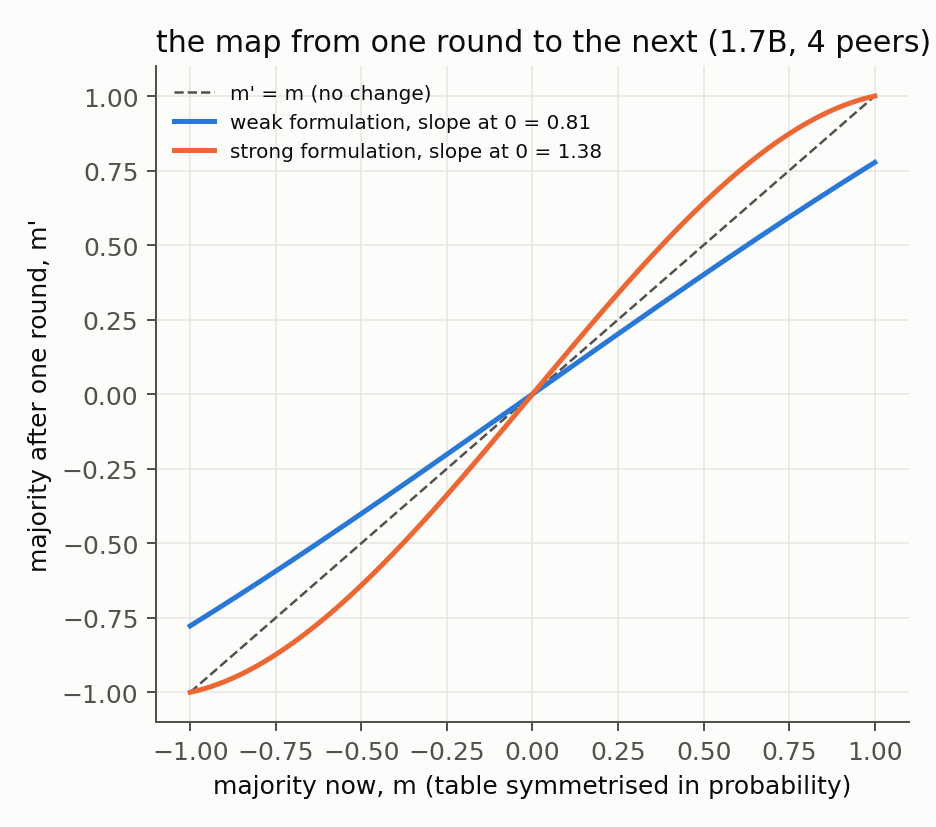
\includegraphics[width=0.62\linewidth]{figL2_map.png}
\caption{What the slope $F'(0)$ looks like on a real table. For two formulations of the 1.7B at 4 peers, the mean-field map $m \to F(m)$: the magnetisation after one round (vertical) against the magnetisation before it (horizontal), from the tabulated policy of each formulation on the table symmetrised in probability, which puts the fixed point back at $m=0$ but keeps the label bias in the slope (Section~3); the dashed line is the identity, where the population stays as it is. The slope of the curve at the centre is $F'(0)$. The orange curve (a strong formulation) crosses the centre steeper than the identity, so a small imbalance grows round after round up to unanimity; the blue one (a weak formulation) crosses it flatter, so a small imbalance shrinks back to the centre. The two formulations run on the same model with the same number of peers; the formulation is what decides the side of the threshold.}
\label{fig:map}
\end{figure}


\paragraph{Protocol.} Each run and each analysis was declared before the data with its cost, hypothesis and decision rule, and a result enters the paper only if it holds in both models, in the paired comparison, with intervals excluding zero and with an independent control. The numbers below are generated from the result files into a registry by a script, and a check rejects any number in the text that is not in the registry. All the declared rules, more than thirty, are listed with their outcomes in Appendix~B. No correction for multiplicity is applied: each finding rests on one pre-declared rule per model, and each control is reported whether it passes or not.

\section{Validation}

The measurement library reproduces the two-dimensional Ising model
(critical point from the peaks of $\chi$ 2.2541 [2.2472, 2.2889] and
from the Binder crossing 2.2673 [2.2614, 2.2718] against 2.2692 exact;
$\gamma/\nu$ 1.7789 [1.7598, 1.7896] against 1.75, an interval that
excludes the exact value because the fit has no correction-to-scaling term
and the bootstrap over seeds measures the statistical error only;
$\beta/\nu$ 0.1197 [0.1115, 0.1322] against 0.125), recovers synthetic $J$
and $h$ with coverage 0.955, 0.950 and 0.945 at the 95\% level (an i.i.d.
bootstrap over synthetic updates, not the cluster interval of the
language-model results), and
reproduces the consensus time of the voter model, proportional to $N^2$ in
single updates, exponent 2.01 [1.96, 2.07]. In population rounds, the unit
of the consensus times below, this is $N\ln 2$ rounds on the complete
graph from a balanced start (5.5, 11.1, 25.0, 44.4 at 8, 16, 36, 64 agents) and of
order $N\ln N$ on the lattice, the drift reference against which every
consensus at small $N$ is read. The finite-size tools validated here are not used in any result on the language models.

With the literal prompt of~\cite{denobili2026} both models reproduce the
field-dominated regime: $\tilde h/\tilde J$ is 14.0 [12.6, 15.9] on the
0.6B and 26.9 [19.7, 46.2] on the 1.7B (he reports about 8 for llama).
With our ten neutral formulations the ratio runs from 0.4 to 50.4 (median
2.5) on the 0.6B and from 0.3 to 3.5 (median 0.8) on the 1.7B, so the regime depends more on the formulation than on the model. At 4 peers $\tilde J$
runs from $-0.04$ to 0.89 across formulations on the 0.6B, with a spread
of 0.35 against a half-width of the 95\% ordering-bootstrap interval of
$\tilde J$ inside a formulation of 0.02, and from 1.04 to 3.26 on the 1.7B
(0.71 against 0.21); up to 4 peers every ordering is enumerated, so inside
a formulation there is no sampling error, that half-width measures the
sensitivity to the set of orderings, and the term of comparison is the
numerical precision. For this reason each coupling is reported together with the formulations it was measured on.

\section{Results}

\begin{figure}[htbp]
\centering
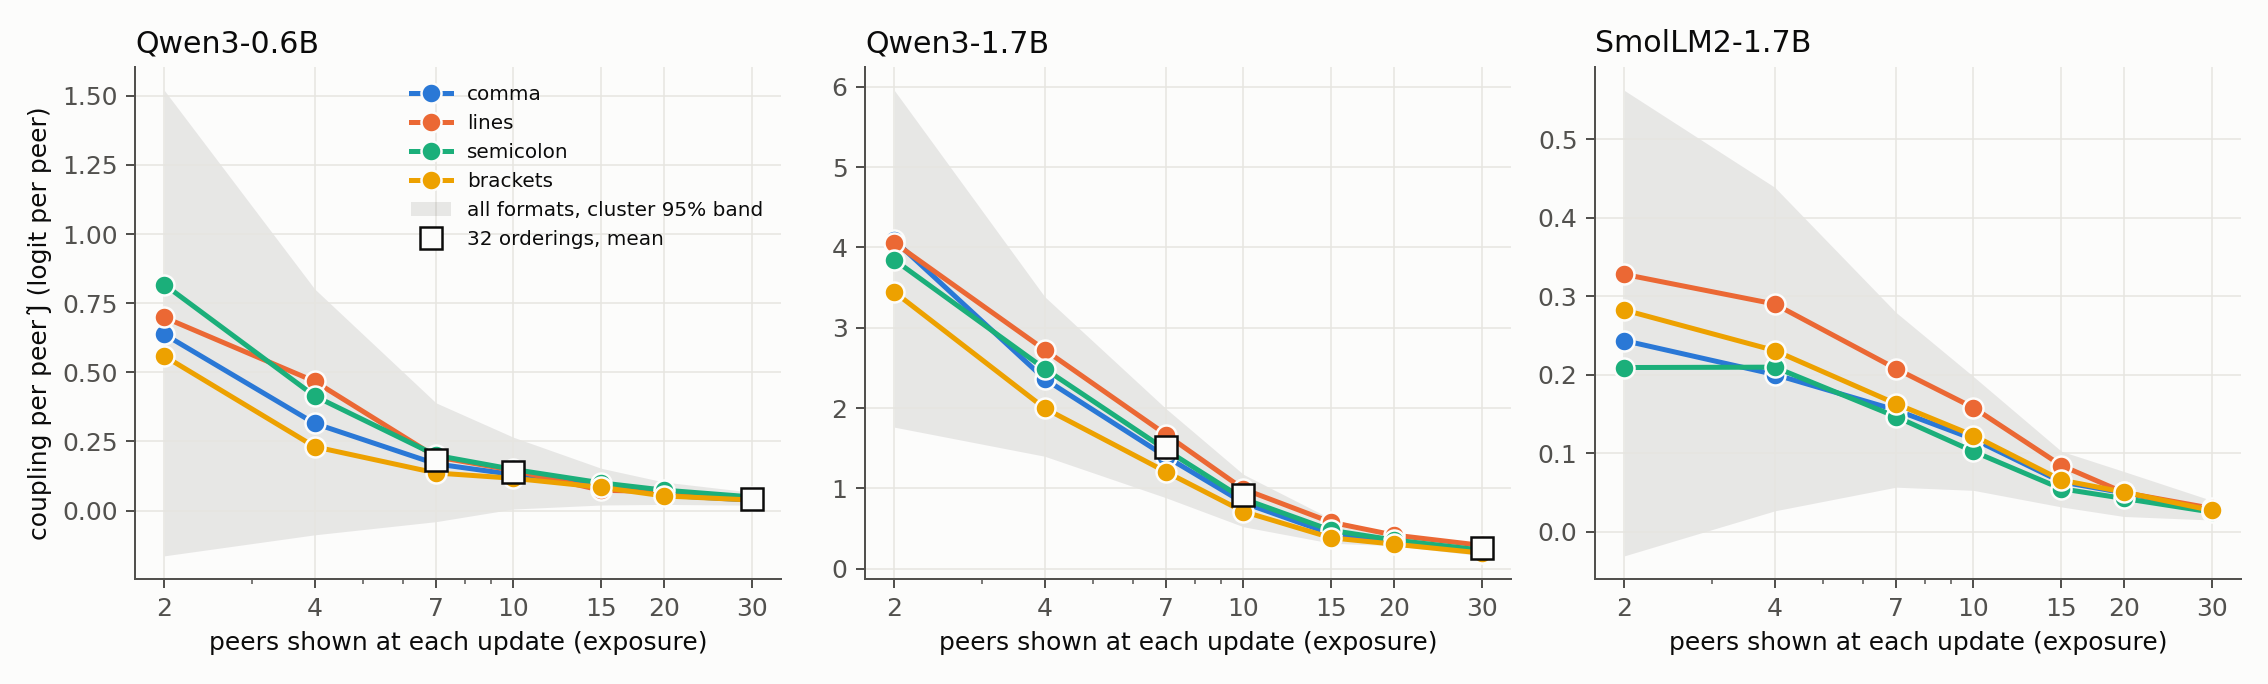
\includegraphics[width=\linewidth]{fig1_coupling_vs_exposure.png}
\caption{Coupling per peer $\tilde J$ against the number of peers shown,
for the three models; one line per list format (mean over the five
wordings), grey band the 95\% $t$ interval on the five per-wording means
on all formats, hollow squares from the 32-ordering tables. All the lines fall; the lines of the different formats lie inside each other's bands, and the squares lie on the lines; the vertical scales differ by a factor of about ten between the
1.7B and the other two models.}
\label{fig:exposure}
\end{figure}

\paragraph{The coupling per peer falls with the number of peers shown.}
The paired difference of $\tilde J$ between exposures is negative in
both models (Figure~\ref{fig:exposure}); $t$ intervals on the per-wording
means. On the ten wordings, from 2 to 7 peers: $-$0.45 $[-0.73, -0.18]$ on the
0.6B (negative in 9/10) and $-$1.76 $[-3.02, -0.50]$ on the 1.7B
(8/10); from 2 to 4 peers $-$0.26 $[-0.44, -0.09]$ and $-$0.90 $[-2.01, 0.21]$,
where the step to 4 peers does not exclude zero on the 1.7B. The five new wordings alone, from 2 to 4 and from 2 to 7 peers: $-$0.25 $[-0.48, -0.02]$ and $-$0.42 $[-0.75, -0.08]$ on the 0.6B,
$-$0.28 $[-2.15, 1.59]$ and $-$0.98 $[-2.90, 0.94]$ on the 1.7B, where they couple less
than the original ones (1.71 against 2.54 at 4 peers). On the five
original wordings alone the interval includes zero on the 0.6B
($-$0.49 $[-1.11, 0.14]$; two of its wordings have $\tilde J$ near zero at every
exposure) and excludes it on the 1.7B from 2 to 7 ($-$2.54 $[-4.73, -0.35]$); the two further separators of the original wordings serve as a robustness check and do not count as a replication. The count channel gives the same direction in its
means.

The total push separates the models (Table~\ref{tab:exposure}). On the 1.7B
$\bar z\tilde J$ grows to 10.64 at 7 peers, falls between 7 and 15
(paired difference $-$3.03 $[-5.19, -0.86]$ over twenty formulations, $t$
interval on the per-wording means; $-$3.04 $[-6.07, -0.02]$ between 7 and 30, marginal) and is then
flat: 9.22 at 10 and 7.60, 7.61, 7.72 at 15, 20 and 30. The unanimity jump,
exact with respect to orderings, is flat from 7 peers on: the ratio between
30 and 7 peers is 1.01 [0.89, 1.15], the exponent
of the jump against the number of peers from 7 on is 0.01 $[-0.08, 0.13]$,
and a model with the fraction of agreeing peers beats a model with their
count in 10 of 10 formulations, with a count coefficient of $-0.02$
$[-0.10, 0.06]$, so from 7 peers on the larger model responds to the fraction of its peers that agree. To be precise, the jump is constant from 7 peers on and the linear push only from 15. The two estimators diverge because
$\tilde J$ is the slope of a linear fit over all $k$ of a response that is
sigmoidal in the fraction $k/e$: as $e$ grows the points crowd near $k=0$
and the slope per peer times $e$ converges to the slope in the fraction,
while the jump measures the total between the extremes. On the 0.6B the
push stays between 1.21 and 1.56 from 2 to 30 peers, with paired
differences between 7 and 15 and between 7 and 30 compatible with zero
(0.07 $[-0.53, 0.67]$ and 0.06 $[-0.82, 0.95]$); the jump of its weak
formulations keeps growing, so we do not claim constancy for this model.

\begin{table}[htbp]
\centering
\caption{Total push and mean-field criterion by exposure, ten
formulations per cell; 32 orderings from 7 peers on. Ceiling
$\mathbb{E}_0|k|$ of $F'(0)$ and mean ratio to it (in brackets, the
formulations within 0.01 of the ceiling); classes from the ordering
interval of $F'(0)$ on the symmetrised map (ordered / disordered /
undetermined) and from the fixed points of the sector-A map (bistable /
field-dominated / disordered; on the 32-ordering tables from 7 peers on). $^{*}$bfloat16 error propagated; one formulation marginal by construction (copy of the first peer). $^{\dagger}$one of the four bistable formulations is that same copy of the first peer, whose map is the identity: 3 + 1 marginal. $^{\ddagger}$one of the nine disordered formulations is within 0.02 of 1.}
\label{tab:exposure}
\small
% generated by scripts/paper_tables.py from paper/numbers.json; do not edit
\begin{tabular}{llcccccc}
\toprule
Model & Peers & $\bar z\tilde J$ & $F'(0)$ & ceiling & ratio (at ceiling) & sym. classes & sector-A classes \\
\midrule
Qwen3-0.6B & 2 & 1.34 & 0.53 & 1.00 & 0.53 (0/10) & 0/10/0 & 0/6/4 \\
Qwen3-0.6B & 4 & 1.56 & 0.56 & 1.50 & 0.37 (0/10) & 1/9/0$^{\ddagger}$ & 1/5/4 \\
Qwen3-0.6B & 7 & 1.27 & 0.46 & 2.19 & 0.21 (0/10) & 1/9/0 & 0/6/4 \\
Qwen3-0.6B & 10 & 1.40 & 0.53 & 2.46 & 0.22 (0/10) & 1/9/0 & 0/6/4 \\
Qwen3-0.6B & 30 & 1.30 & 0.54 & 4.33 & 0.13 (0/10) & 1/9/0 & 1/6/3 \\
Qwen3-1.7B & 2 & 8.14 & 0.89 & 1.00 & 0.89 (7/10) & 0/10/0 & 0/10/0 \\
Qwen3-1.7B & 4 & 10.17 & 1.15 & 1.50 & 0.76 (0/10) & 6/1/3$^{*}$ & 4/6/0$^{\dagger}$ \\
Qwen3-1.7B & 7 & 10.64 & 1.45 & 2.19 & 0.66 (0/10) & 8/1/1 & 8/2/0 \\
Qwen3-1.7B & 10 & 9.22 & 1.39 & 2.46 & 0.57 (0/10) & 7/2/1 & 7/3/0 \\
Qwen3-1.7B & 30 & 7.72 & 1.35 & 4.33 & 0.31 (0/10) & 5/2/3 & 8/2/0 \\
\bottomrule
\end{tabular}

\end{table}

\paragraph{The mean-field criterion.} The linear criterion $\bar z\tilde J>1$
puts 10 of 10 formulations of the 1.7B and 6 of 10 of the 0.6B above
threshold at every exposure. The slope $F'(0)$ of the mean-field map on the
table does not assume linearity in $k$ and gives a different picture
(Table~\ref{tab:exposure}, Figure~\ref{fig:classes}), read against the
ceiling. At 2 peers the ceiling is 1 and no formulation can be ordered:
the 1.7B has 7/10 formulations within 0.01 of it, at the noiseless
majority rule, so the count of zero ordered formulations at 2 peers comes from sampling only two peers and says nothing about the model. From 4 peers on the ceiling lies above 1 and a classification is possible: the 0.6B has at most one ordered formulation at any
exposure and the 1.7B a majority at 4 to 10 peers and half at 30, while
its ratio to the ceiling falls at every exposure. At 4 peers the 1.7B is
in bfloat16 with every ordering enumerated, so the numerical error is the
one to propagate: with a Gaussian error of 0.37 logit (the mean of the two
standard deviations of the float32 check) on every gap, 7 of
10 formulations stay above 1 in at least 97.5\% of 400 draws, 1 below and
2 are undetermined; one further formulation (wording 4, comma) copies
the first peer listed in every configuration, a policy whose map is the
identity and $F'(0) = 1$ by construction, so the defensible count at 4
peers is 6 ordered, 1 disordered and 3 undetermined. On the 0.6B at 4 peers the one formulation above 1 is joined by one at 0.98, within 0.02 of the threshold; what the small model lacks is not the interaction: on the odd part of its tables the interaction alone is above threshold in four formulations (1.14 to 1.25), at the threshold in two and null or weak in four ($-0.04$ to 0.45), and it is the label bias, through $\mathrm{sech}^2\tilde h$, that brings the slope of the mixed population to 0.56 with one formulation above 1 (Appendix~\ref{app:decomposition}); the formulation with the smallest bias, $\tilde h = 0.29$, is the one that stays above threshold and the only bistable one in sector A. Below threshold on this criterion means that the mixed population does not order, not that the agents ignore their peers. The classes of the labelled population (last column) give information that the symmetrised map does not: on the 1.7B all ten formulations go to
consensus on the label the bias favours at 2 peers, 4/10 are bistable at
4 (one of them the copy of the first peer, marginal by construction) and 8, 7, 8 of 10 at 7, 10 and 30 on the 32-ordering tables (the
class holding in at least 95\% of an ordering bootstrap for 7 to 9 of
10), with none disordered; on the 0.6B
at most one formulation is bistable at any exposure, 5 or 6 of 10 are
field-dominated and 3 or 4 disordered, with single fixed points between
$|m^*| = 0.22$ and 0.87. So a population below threshold can still reach consensus. Spontaneous order, on the other hand, appears in 4 of 10 formulations
of the 1.7B at 4 peers and in most from 7 peers on, and in at most one
formulation of the 0.6B. The criterion was checked for consistency against the tabulated
dynamics of the same table, at 200 agents on the complete graph where the
map is exact up to corrections of order $N^{-1/2}$: the dynamics at 4
peers, 30 seeds and 60 rounds, with the rule written before the data,
agrees with the class in 16 formulations of 20 by the declared rule, the
four disagreements having $F'(0)$ within 0.02 of 1; an exploration at
600 rounds, outside the rule, resolved two in the predicted direction,
one against and one not at all, and the count stays 16 of 20. On the sector-A
table the same dynamics lands within 0.05 of the stable fixed point of
the sector-A map in 19/20 formulations, the seeds splitting between the
branches in the bistable one at $F'(0)=1.00$. One formulation contradicts the linear criterion directly: a formulation of the 1.7B with $\bar z\tilde J$
above 1 and $F'(0)=0.81$ stays disordered at 200 agents with $|m|=0.13$ on
the symmetrised table and goes to unanimity on the favoured label on its
own. The classification is insensitive to the rescaling of the logits: at
scale 0.7 the counts above 1 move by at most one formulation per cell
(1.7B at 4 peers 1.15 to 1.16, 8/10 and 7/10 above 1). The $\beta$ of~\cite{demarzo2026} is the slope of the tanh at $m=0$
and corresponds to $F'(0)$ on the table symmetrised in probability, not to $\bar z\tilde J$ (like a $\beta$ fitted on the adoption curve of a labelled population, this slope includes the flattening by the bias; the slope of the odd part alone is not computed at 30 peers, where the orderings are sampled); in their protocol
every agent sees all 49 others and $\beta$ has no sampling ceiling, so
only our 30-peer row is comparable: there the 1.7B (1.35) sits with the
majority of their models and the 0.6B (0.54) below.

\begin{figure}[htbp]
\centering
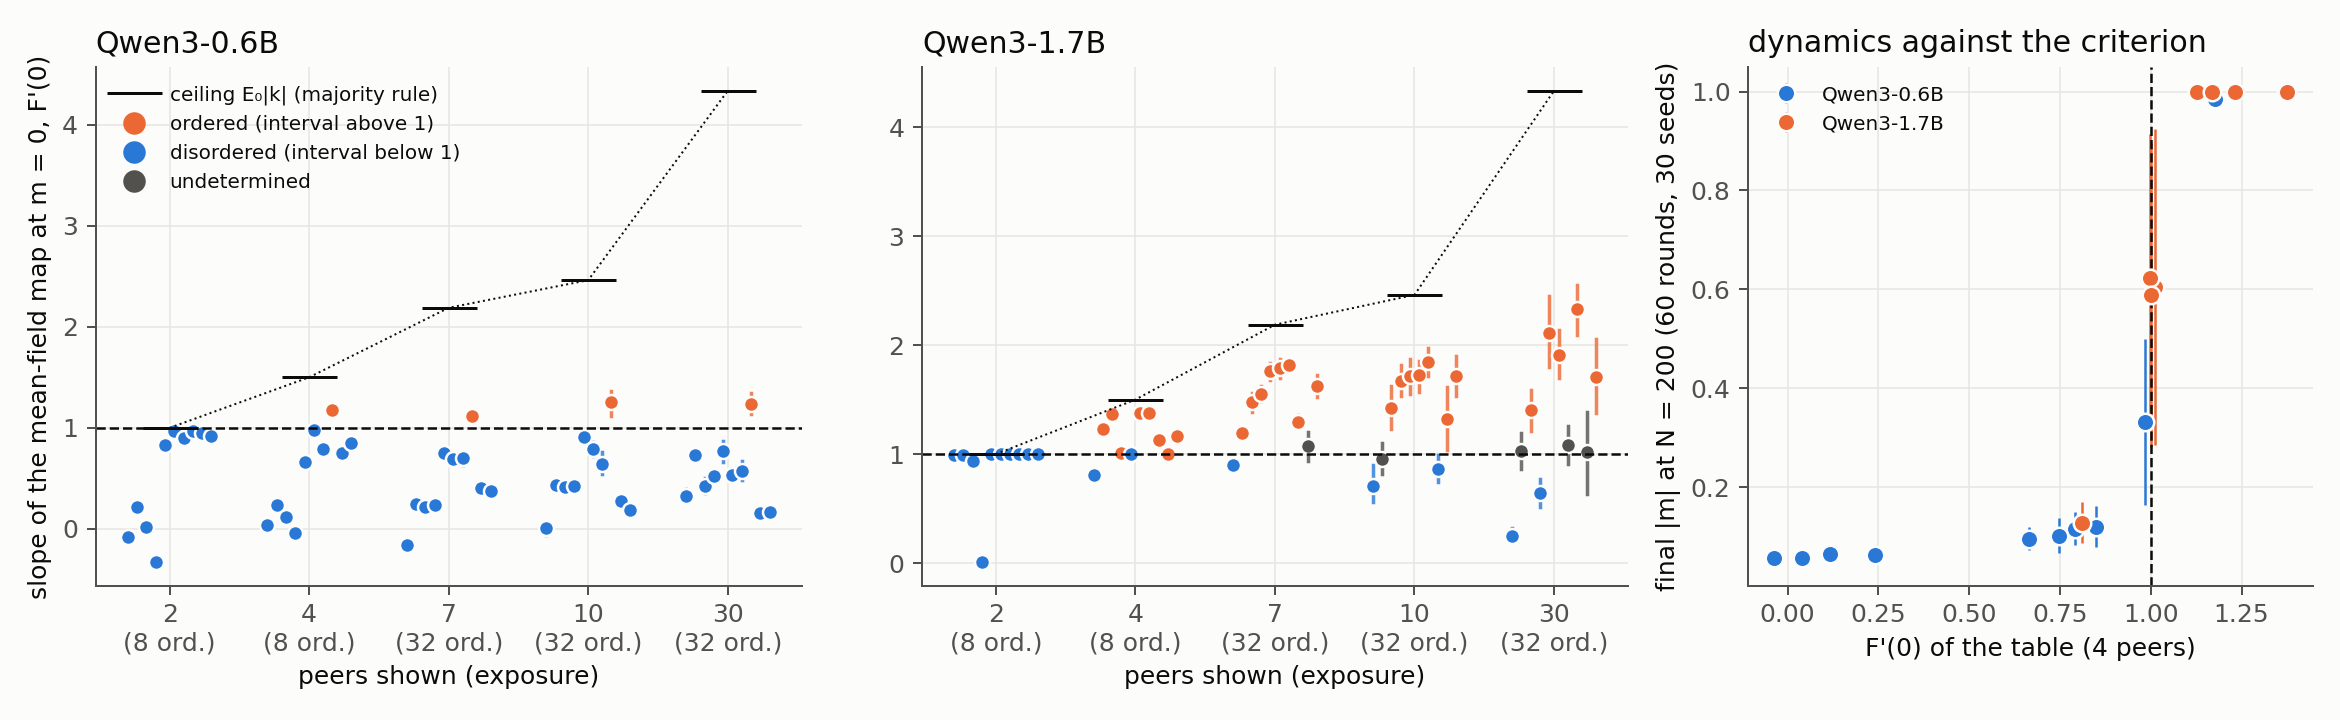
\includegraphics[width=\linewidth]{fig3_meanfield_classes.png}
\caption{Left and centre: $F'(0)$ for every formulation at every exposure
with its interval over the sampled orderings, coloured by class; the
dashed line is the threshold and the short marks are the ceiling
$\mathbb{E}_0|k|$ at each exposure. Right: final $|m|$ of the tabulated dynamics
at 200 agents against $F'(0)$ of the same table at 4 peers.}
\label{fig:classes}
\end{figure}

\paragraph{Precision of the numbers.} Re-tabulating the cells at 7, 10 and
30 peers with 32 orderings moves $\bar z\tilde J$ by $-0.09$ $[-0.16, -0.04]$,
0.15 [0.03, 0.30] and 0.10 [0.04, 0.16] on the 1.7B and by 0.00 $[-0.01, 0.02]$,
0.03 [0.01, 0.04] and 0.04 [0.02, 0.06] on the 0.6B, within 3\%, and
$F'(0)$ is stable in the same way. The shifts share a sign because the 8
orderings are drawn with one seed shared by every formulation of a cell and
by the two models (identical sampled orderings), so the four comparisons
are two draws seen by two models; a subset of 8 orderings is unbiased for
the 32-ordering mean by construction, and random subsets from the
32-ordering tables give a null distribution of standard deviation
0.019 to 0.101 in $\bar z\tilde J$ in which the two independent observed
shifts sit at tail fractions 0.080 and 0.020, the second outside the
central 95\% range: the declared rule is therefore not satisfied strictly. What we keep from this check is that the 8-ordering estimate is unbiased, together with the size of the fluctuation shared by the cells. The 1.7B is tabulated in bfloat16; against float32 on the same cells
the per-gap difference has standard deviation 0.35 to 0.39 logit and
maximum 1.17, three times the error of the 0.6B, and on the full
32-ordering cells at 10 and 30 peers $F'(0)$ in float32 lies inside the
bfloat16 ordering interval in 18 formulations of 20, with the classes
changing by at most one formulation per exposure.

\begin{figure}[htbp]
\centering
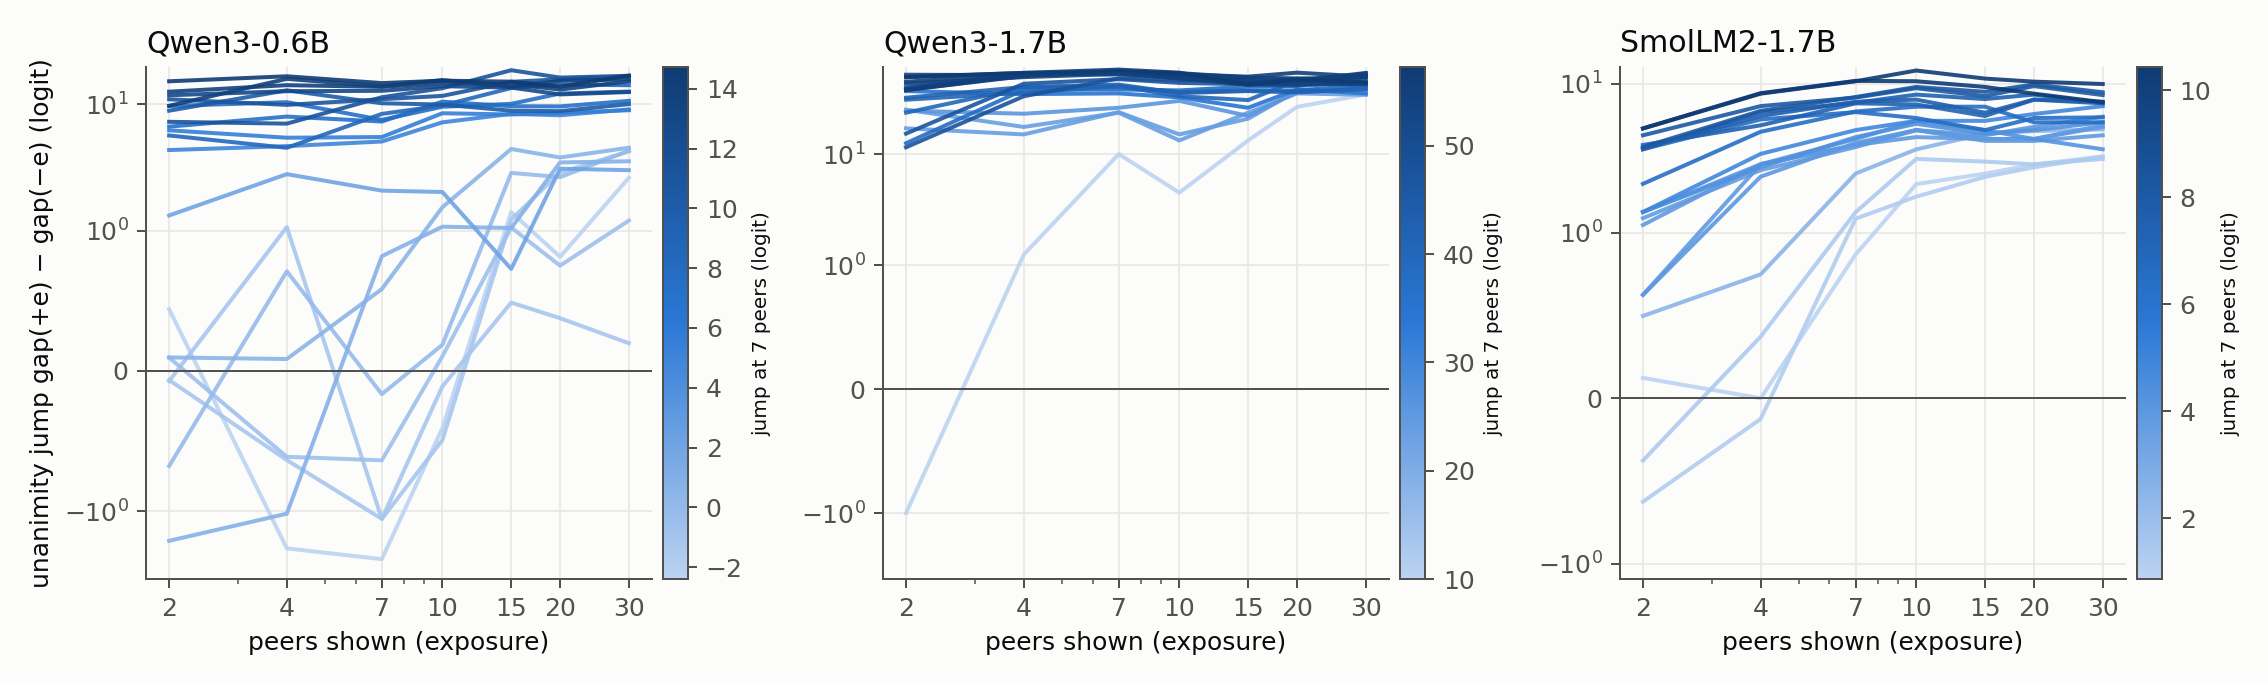
\includegraphics[width=\linewidth]{fig2_jump_vs_exposure.png}
\caption{Unanimity jump against the number of peers, one line per
formulation coloured by the jump at 7 peers (light: weak, dark: strong),
symmetric log scale. A flat line means the jump has stopped growing with the number of peers; a rising line means it is still growing.}
\label{fig:jump}
\end{figure}

\paragraph{The shape of the response depends on the coupling strength of
the formulation.} The exponent of the unanimity jump against the number of
peers from 7 to 30 (0 for a response to the fraction, 1 for a response to
the count) varies across formulations and is exact per formulation. It
correlates with the strength of the formulation (Figure~\ref{fig:jump}):
Spearman's correlation with the jump at 7 peers is $-0.72$ $[-0.89, -0.16]$
($p = 0.002$, $n = 15$) on the 0.6B, $-0.88$ $[-0.95, -0.28]$ ($p < 0.001$,
$n = 20$) on the 1.7B and $-0.78$ $[-0.93, -0.35]$ ($p < 0.001$, $n = 20$)
on SmolLM2-1.7B; with disjoint points (exponent on 10 to 30 peers against
the jump at 2 peers) $-0.69$ $[-0.96, -0.08]$, $-0.65$ $[-0.86, -0.08]$
and $-0.64$ $[-0.80, -0.28]$. Splitting the formulations at the median of
the jump at 2 peers, the mean exponent of the weak half minus the strong
half is 0.44 [0.11, 0.96], 0.34 [0.06, 0.64] and 0.39 [0.14, 0.64]; with
the exponent from 10 peers the split fails its rule on the 0.6B
(0.37 $[-0.01, 1.03]$). These $p$ values count formats inside five
wordings; at the wording level ($n = 5$) the correlation is $-$1.00
(exact $p$ 0.017), $-$0.90 (0.083) and $-$0.80 (0.133),
significant at 5\% in the small model only. Two null models reproduce the
regularity: on the 0.6B the absolute increment of the jump between 7 and
30 peers does not depend on the strength (Spearman $-$0.15, $p$ 0.52),
and a common additive increment gives Spearman $-$1.00 and a split of
0.52 against 0.57 observed; on the two larger models the strong half
has negative increments ($-$5.34 and $-$0.45 against
6.31 and 1.72), a ceiling. We therefore report the regularity as descriptive only: in proportion, weak formulations grow more than strong ones with the number of peers.
It was found on the ten original formulations and then written as a
prediction before the two further separators (no new cluster) and before
the twenty formulations of SmolLM2, the only out-of-family test. The jump of the 1.7B is
saturated in probability ($P(+\mid +e)$ and $P(-\mid -e)$ above 0.99) in
17 to 20 of 20 formulations from 7 peers on, in 0 to 5 on the 0.6B and at
most 1 on SmolLM2, so the flat jump and its exponent are properties of the logit gap in a range where a generating agent already follows unanimous peers, whereas the growth of the weak formulations happens where the probability still moves, which is the range measured by~\cite{bellina2026}. On the 0.6B the dispersion of
the jump across formulations does not shrink from 7 to 30 peers (ratio
0.98), as the additive null predicts. We do not claim any functional form for the response.

\begin{figure}[htbp]
\centering
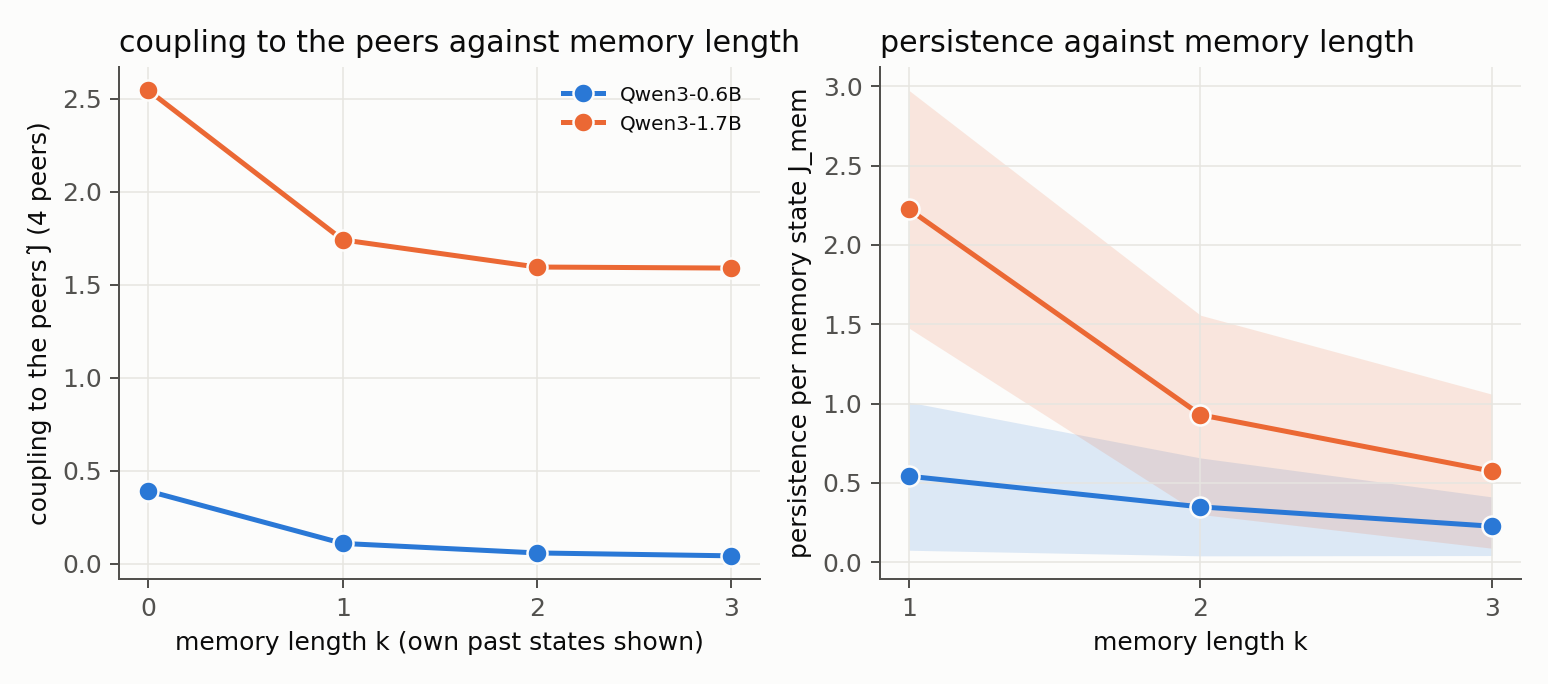
\includegraphics[width=\linewidth]{fig4_memory_curve.png}
\caption{Left: coupling to the peers against the memory length at 4 peers.
Right: persistence per memory state with the 95\% $t$ interval on the
per-wording means as a band.}
\label{fig:memory}
\end{figure}

\paragraph{Memory of one's own past states reduces the coupling to the
peers.} With memory of three previous states, $\tilde J$ to the peers falls
in both models at 4 peers (Figure~\ref{fig:memory}): on the ten wordings
$-$0.30 $[-0.46, -0.14]$ on the 0.6B and $-$0.83 $[-1.09, -0.56]$ on the 1.7B; on the five
new alone $-$0.25 $[-0.45, -0.06]$ and $-$0.70 $[-1.30, -0.10]$; on the five original
alone $-$0.35 $[-0.72, 0.02]$ and $-$0.95 $[-1.16, -0.75]$. The sign is
the opposite of the expectation written in the plan before the
measurements; the pre-registered curve in the memory length confirms it:
$\tilde J$ is 0.39, 0.11, 0.06, 0.04 at $k = 0,1,2,3$ on the 0.6B and 2.54,
1.74, 1.59, 1.59 on the 1.7B, with paired steps $-$0.28 $[-0.60, 0.04]$,
$-$0.05 $[-0.09, -0.02]$, $-$0.02 $[-0.04, 0.01]$ and $-$0.80 $[-1.05, -0.56]$,
$-$0.15 $[-0.29, -0.00]$, $-$0.01 $[-0.11, 0.10]$: non-increasing, with the first
remembered state carrying the effect. The count channel replicates the sign
with five wordings ($-$0.30 $[-0.49, -0.11]$ and $-$0.54 $[-1.25, 0.18]$, the latter
including zero). Memory adds a
persistence term, the coefficient of the sum of the memory states, which
measures how much the model repeats its own states and must be kept
distinct from conformity to the history of the peers: per state it is
0.54, 0.35, 0.23 on the 0.6B and 2.22, 0.93, 0.57 on the 1.7B at
$k = 1, 2, 3$, falling in the mean at every step, the steps excluding zero on
the 1.7B and only the total from $k=1$ to 3 on the 0.6B; paired steps $-$0.19 $[-0.39, 0.00]$, $-$0.12 $[-0.25, 0.01]$ and
$-$1.29 $[-1.69, -0.90]$, $-$0.36 $[-0.53, -0.18]$.
Persistence enters the instability of the disordered state with the same
sign as the coupling to the peers: linearising around $m=0$, the threshold
of the combined linear gain is $e\tilde J + k J_{\text{mem}} = 1$. At 4
peers that gain is 1.56, 0.98, 0.93, 0.85 at $k=0,1,2,3$ on the 0.6B
and 10.17, 9.19, 8.24, 8.08 on the 1.7B: memory moves coupling from
the peers to the agent itself and reduces the total gain by 45\% and
21\% at $k=3$, without changing the side of the threshold of the
larger model at any exposure. At $k=1$, where the memory is the own
previous state, the round map $m \mapsto \mathbb{E}[2P(+\mid k, s)-1]$ with
$s$ drawn at the same magnetisation gives $F'(0) = $ 0.55 on the 0.6B
(0/10 above 1) and 1.36 on the 1.7B (9/10), against 0.56 and
1.15 at $k=0$: memory does not change the side of the threshold,
and on the larger model the slope rises, because the own state enters the
round map with the sign of the peers. Beyond $k=1$ the slope is not
computed. With four unanimous peers against the own last state, the peers
win on the 1.7B ($P(+\mid k=+4, \text{mem}=-1)$ from 0.88 to 1.00)
while on the 0.6B the own state wins in 10/10 formulations when it is A
($P(+\mid k=-4, \text{mem}=+1)$ from 0.60 to 0.98). In a cell with an explicit decisional instruction, declared after the main analysis, the own state still prevails in 8/10 formulations and $J_{\text{mem}}$ is unchanged (0.42 to 0.41,
paired $-$0.01 $[-0.20, 0.17]$), so the effect is persistence and is not a recall induced by the instruction.

\paragraph{The list separator has no detectable effect on the coupling, whereas the presentation of the peers (list against count) has one.} In a mixed model on $\tilde J$ with a random intercept per wording and a
variance component for the wording by format pair, likelihood-ratio tests
on 140 rows per model give for the format LR 0.62 on 3 degrees of
freedom ($p = 0.891$) on the 0.6B, 1.63 ($p = 0.654$) on the 1.7B and
1.16 ($p = 0.764$) on SmolLM2, and for the interaction LR 4.14, 3.15
and 5.26 on 18 degrees of freedom (a first version without the pair
component gave $p = 0.384$, 0.160 and 0.042, anticonservative)
(Figure~\ref{fig:format}). The minimum detectable effect, from the paired
contrasts against the comma list with $t$ intervals over wordings, is
about a tenth of $\tilde J$ on the 0.6B and three tenths on the 1.7B. The means by format at 2
peers span 0.56 to 0.82 on the 0.6B and 3.44 to 4.09 on the 1.7B, a few
tenths where the exposure moves $\tilde J$ by a factor of ten. All four formats are separators of the same list. The only change of presentation in the data, the count channel against the comma list, does move the coupling: $\tilde J(\text{count}) - \tilde J(\text{list})$ over the five
wordings is $-$1.03 $[-2.38, 0.07]$, $-$0.86 $[-1.35, -0.42]$ and
$-$0.59 $[-0.90, -0.24]$ at 2, 4 and 7 peers on the 1.7B and 0.23 $[-0.06, 0.48]$,
0.11 $[-0.05, 0.23]$ and 0.03 $[-0.05, 0.11]$ on the 0.6B, the direction~\cite{cho2025}
report for the format of the peers.

\begin{figure}[htbp]
\centering
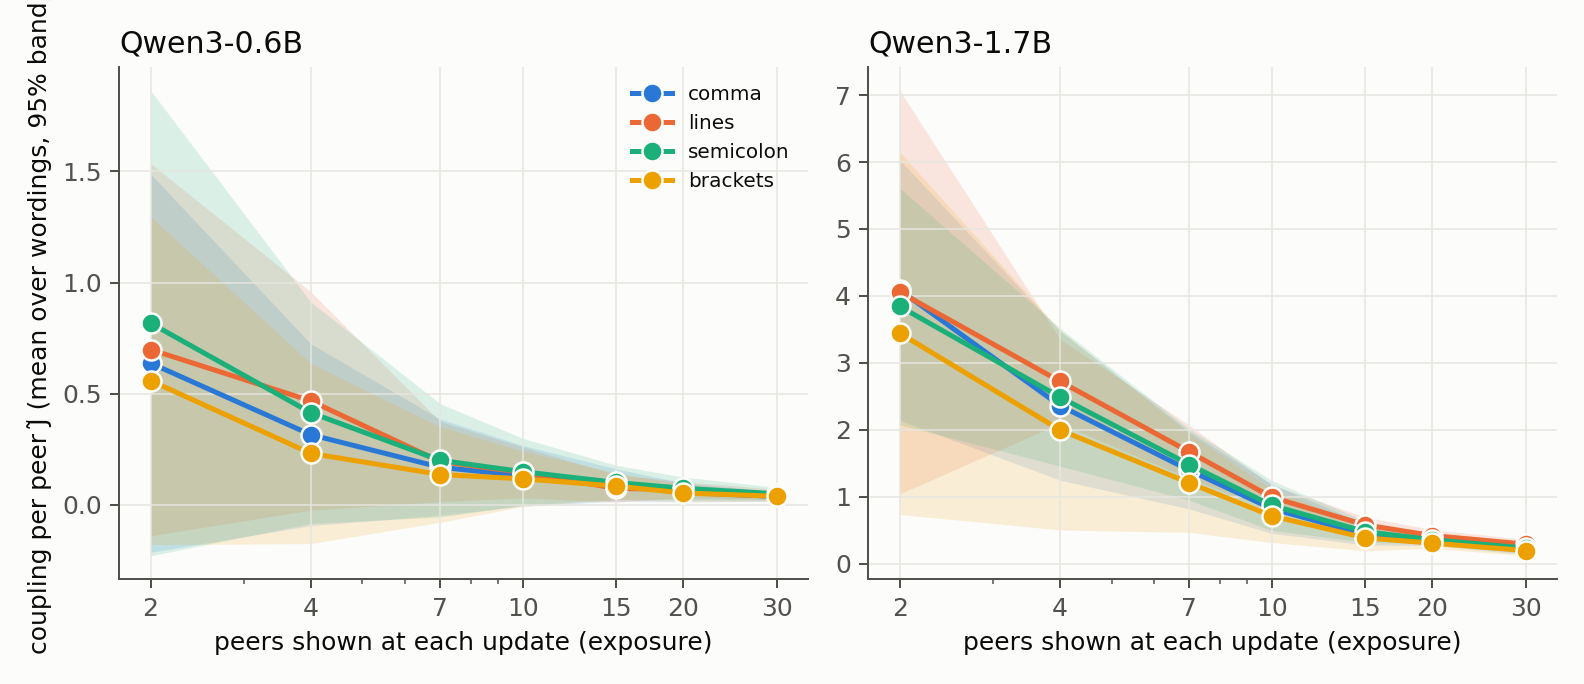
\includegraphics[width=\linewidth]{fig6_format.png}
\caption{Coupling per peer by list format with the 95\% $t$ band of each
format over the five wordings; the bands overlap at every exposure.}
\label{fig:format}
\end{figure}

\paragraph{Controls.} At these couplings the lattice control does not
discriminate the topology: the 1.7B at 4 peers has $\tilde J = 2.54$ per
peer against a mean-field threshold of 0.25 and an Ising threshold of
0.44 on the square lattice, and the 0.6B has $F'(0) = 0.56$ with a bias $\tilde h = 0.81$, that is $2\tilde h$ above one and a half logit, so the fractions of runs reaching consensus at
36 agents are the same on both graphs (0.71 and 0.71 on the 0.6B, 0.99 and
1.00 on the 1.7B). On the 1.7B, where every run reaches consensus, the
consensus time in rounds on the complete graph is below the drift
reference $N\ln 2$ at every size (2.7, 4.8, 7.6, 9.6 rounds against
5.5, 11.1, 25.0, 44.4 at 8, 16, 36, 64 agents, below drift in 10, 10, 9, 10
formulations of 10); the median formulation is nearly flat in $N$, the
logarithmic escape of an ordered phase, and one formulation near threshold
grows like drift. On the lattice the drift reference grows as $N\ln N$ and
coarsening also grows with $N$, so the lattice exponent does not separate
interaction from noise. On the 0.6B the fraction of runs reaching consensus
falls with $N$ (0.98, 0.88, 0.71, 0.63 at 8, 16, 36, 64 agents), the drift
of the voter reference at small $N$, and the runs that reach it at 8 agents
take 7.6 rounds against 5.5 of drift. Hysteresis under stubborn agents is
a qualitative control at 8 agents, where the step of the stubborn fraction
is one agent and the gap at zero stubborn agents measures the stability of
the absorbing consensus over the 20 rounds of the sweep: the up branch of
the 1.7B tips at one or two stubborn agents in 9 formulations of 10 and
the down branch in 8, the rest held by the bias, and the tipping fraction
is not estimable at this resolution. The gap under stubborn agents placed
at random persists on the lattice (1.68 against 1.86 on the 1.7B, 0.48
against 0.72 on the 0.6B), while a contiguous placement collapses it (Figure~\ref{fig:controls}).

\begin{figure}[htbp]
\centering
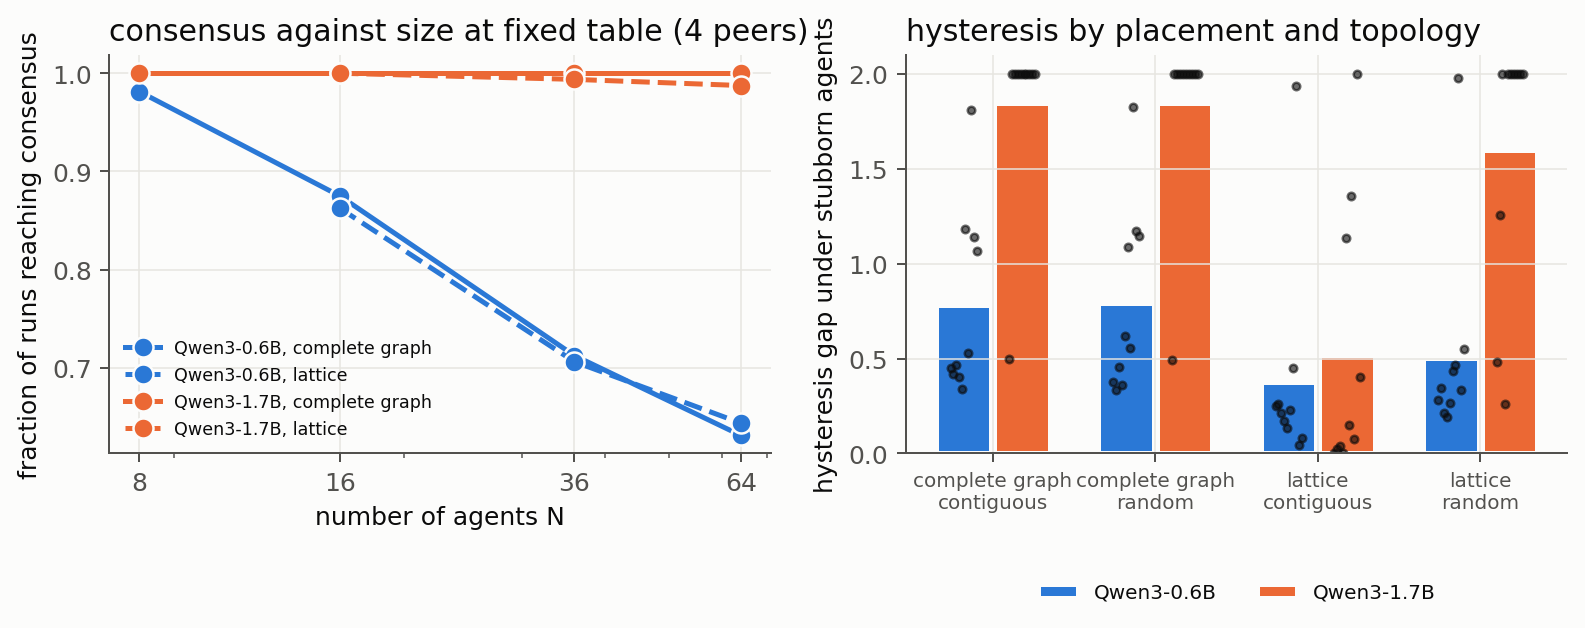
\includegraphics[width=\linewidth]{fig5_controls.png}
\caption{Controls. Left: fraction of runs reaching consensus against the number of agents $N$, at fixed table (4 peers), on the complete graph and on the lattice; a curve that stays at 1 means the population orders at every size, which is the work of the interaction; a curve that falls with $N$ means the population reaches consensus only when it is small, which is the work of the noise. Right: hysteresis gap under stubborn agents by placement (contiguous rows against random) and topology, bars for the mean over formulations, dots for the formulations; the contiguous placement on the lattice collapses the gap and the random placement restores it, a qualitative reading at the resolution of one stubborn agent.}
\label{fig:controls}
\end{figure}

\section{Limitations}

Everything above is measured on the Qwen3 family at 0.6 and 1.7 billion
parameters, in an abstract game without ground truth, at the poor channel,
with a fixed rescaling of the logits, on ten shared formulations (twenty
for the exposure and format results). We have not measured a channel with generated text, a designed specification field, or a task with a ground truth; we have only two model sizes (two replications, not a curve) and two families, memory only up to $k = 3$, and no topology other than the lattice and the complete graph. Nothing measured here extends to models two or three orders of magnitude larger: the threshold structure survives at that scale (Okawa on GPT 4.1, DeepSeek V3, Llama 3.1 from 8B to 405B, Mistral and Qwen3 235B; Ashery and co-authors on Llama-70B and Claude 3.5 Sonnet) but the sign of the coupling can change with the family (Okawa fits a negative conformity parameter to the GPT 4.1 variants, anticonformity in a spin model, and a positive one to Llama 3.1 and to the Qwen3 235B base model, his Instruct variants deviating from the base ones), and two models of one family at a factor three in size already sit on opposite sides of the threshold here. The values have to be measured again on the model in use; the method, the map and the criterion carry over, the values do not.

The second family, SmolLM2-1.7B-Instruct, enters the result on the shape of
the response, where the prediction was written before its data; for the
decrease of the coupling between 2 and 7 peers the declared rule did not
hold (paired differences $-0.03$ $[-0.10, 0.03]$ and $-0.10$ $[-0.21, 0.02]$
on twenty formulations); its coupling per peer is 0.286, 0.245, 0.181, 0.138, 0.074, 0.050 and 0.029 at 2 to 30 peers, a fall from 7 to 30 of the same order as in the Qwen models, which was not the declared test and which we do not claim,
and its mass on the label tokens is lower (cell means 0.949 to 0.987).
That result holds for the Qwen family only, and the second family counts as a limitation of it. A third family was deferred; it would widen or narrow the scope of that result without changing any of the numbers reported here.

The wording is the independent unit, five original and five new; every interval that supports a finding is a $t$ interval on the per-wording means, and effects below its half-width are not detectable. A replication independent of the original
family requires new wordings, which the five new ones are for the exposure
and memory findings. From 7 peers on the grid samples 8 orderings per sum with one seed shared
by all formulations; the cells at 7, 10 and 30 peers were re-tabulated with
32, and the paired differences between exposures at 8 orderings carry a
common error of the order of one to two percent that the intervals do not
include; no threshold is within that margin. $R^2$ of the linear fit in $k$
rises with the number of orderings and is not used. The 1.7B is tabulated
in bfloat16 with the per-gap error measured above. The memory in the
dynamics is initialised by repeating the initial state; the fitted
quantities enumerate every memory tuple and do not depend on it. The
persistence per state assumes equal weights of the memory states, an
approximation: a control against the full memory state finds the memory
acting as a complete state in the 0.6B and with unequal position weights
in the 1.7B. The policy is a first-token conditional after an imposed
prefix, without thinking and without a system prompt: whether the model
produces the prefix in free generation, the thinking mode, and truncated
sampling are not covered, and the correspondence with what an agent
writes was checked on two formulations at 4 peers (Setup). With the mean token loss of the prompt as a
regressor the variance of $\tilde J$ across wordings on the 1.7B falls
from 0.362 to 0.195 ($p = 0.031$), on five wordings a
descriptive fact (Appendix~A). The mean-field slope with memory is
computed at $k=1$ only, and beyond $k=1$ there is only the combined linear gain; the symmetrised table serves the
map and the consistency check, the sector tables the grid dynamics;
hysteresis is read at the resolution of one stubborn agent and the lattice
control runs at couplings where the topology is not discriminated. The
shape of the response of the small model to the number of peers is not
determined by any single functional form. The coupling varies by an order of magnitude with the formulation; the paired design is what protects the comparisons against this variation.

\section{Reproducibility}

All the runs were made on one consumer laptop CPU with 16 GB of memory; the
tabulation of one cell takes minutes to hours depending on the exposure
and the population dynamics runs in seconds. Code, one configuration file
per cell (with the precision and the HuggingFace revision of the weights),
manifests with revision, precision, seeds, commit hash and the state of the
working tree, the raw gap tables, every measure file and a pinned
\texttt{requirements.txt} accompany the paper in the public repository,
\url{https://github.com/PhysicsInforMe/subcritical-agents}. A driver
(\texttt{scripts/reproduce.py}) lists every analysis with the exact
arguments recorded in the manifest of its output and, in check mode,
reruns the chain in a copy and reports whether each regenerated file
equals the committed one outside the manifest; the model runs and the
long dynamics are its inputs, not repeated; the precision-check cells have
their own configuration files with the precision they were run at. As stated in the Protocol paragraph, the numbers in the text and in the two tables are generated from those files into a registry by a script and checked against the text, and each run was declared in the project log before the data with its cost, hypothesis and rule.

\section{Conclusion}

Showing an agent more peers does not couple it more strongly to each of them. The coupling per peer falls, and in the larger model the unanimity jump is flat from 7 peers on and the linear push from 15, so the agent responds to the fraction of its peers that agree. In that model, then, a smaller exposure does not protect against collective order, and a larger one does not increase the pull beyond 7 peers. Which side of the threshold a population sits on
is decided by $F'(0)$ on its tabulated first-token policy, a quantity that costs one
forward pass per configuration and that we checked for consistency against
the dynamics of the same table; the linear summary overestimates order, and
the criterion has a ceiling set by the number of peers sampled, so it
separates the models from 4 peers on. Below threshold does not mean a weak interaction: at 4 peers the interaction of the 0.6B alone, read from the odd part of its tables, is at or above threshold in six formulations of ten, and it is the label bias that flattens the response of the mixed population by $\mathrm{sech}^2\tilde h$ (Appendix~\ref{app:decomposition}). A population below threshold can still reach consensus: the labelled population of the 0.6B reaches unanimity on the
label its bias favours in five or six formulations of ten, and at 16
agents or fewer drift alone produces consensus in about $N\ln 2$ rounds. Spontaneous order, the bistable class, is what the 1.7B shows in 4 of 10 formulations at 4 peers (one of them marginal by construction) and in most from 7 peers on, and the 0.6B in at most one formulation at any exposure. Memory of one's own past
states moves coupling from the peers to the agent itself, reducing the
combined gain by a fifth on the 1.7B and by nearly half on the 0.6B, while
the mean-field slope at $k=1$ does not fall and rises on the 1.7B,
without crossing the threshold in any measured cell; the cost is that the agents repeat their own past states. At this precision the list separator does not act as a knob, while the presentation of the peers, list against count, does in the larger model. The prompt formulation is a first-order knob, and a coupling has to be reported with the formulations it was measured on. The next phase will add the field axis, a designed specification that competes with the peers, and the accuracy on a task with a ground truth.

\clearpage
\appendix
\section{The ten wordings}
\label{app:wordings}

Slots: \{a\} \{b\} \{n\_peers\} \{peers\} \{memory\}; the memory slot is
empty at $k=0$. The text is what the model reads before the imposed
prefix \texttt{\{"state": "}.

\noindent\textbf{Wording 0.} \texttt{Player 1 is one of several players. Each player holds a state, either \{a\} or \{b\}. Player 1 sees \{n\_peers\} other players and their states are: \{peers\}.\{memory\} Answer with the state Player 1 should hold now, as JSON with a single key "state".}

\noindent\textbf{Wording 1.} \texttt{In this game every player has a state, \{a\} or \{b\}. Player 1 can see the states of \{n\_peers\} other players: \{peers\}.\{memory\} Reply with the state that Player 1 takes now, in JSON with the key "state".}

\noindent\textbf{Wording 2.} \texttt{Player 1 takes part in a game where each participant holds one of two states, \{a\} or \{b\}. The states of the \{n\_peers\} players Player 1 can see are: \{peers\}.\{memory\} Give the state Player 1 should adopt now as a JSON object with the single key "state".}

\noindent\textbf{Wording 3.} \texttt{Each player in the game is in state \{a\} or in state \{b\}. Player 1 observes \{n\_peers\} other players with these states: \{peers\}.\{memory\} State Player 1 should now be in, as JSON with one key called "state".}

\noindent\textbf{Wording 4.} \texttt{Consider Player 1 among a group of players whose state is either \{a\} or \{b\}. The current states of the \{n\_peers\} players visible to Player 1 read: \{peers\}.\{memory\} Output the state Player 1 holds now as JSON containing only the key "state".}



\medskip
\noindent\textbf{The five new wordings (written after the first five had been analysed).}

\noindent\textbf{Wording 5.} \texttt{Reply as JSON with the single key "state". You are Player 1 in a game where every player is in state \{b\} or in state \{a\}. You can see \{n\_peers\} other players and their states are: \{peers\}.\{memory\} Decide the state you take now.}

\noindent\textbf{Wording 6.} \texttt{Return a JSON object with one key, "state", giving the state of Player 1. The game has two states, \{a\} and \{b\}. \{n\_peers\} other players are visible to Player 1 and they hold: \{peers\}.\{memory\} Report the state of Player 1 now.}

\noindent\textbf{Wording 7.} \texttt{There are two possible states, \{b\} and \{a\}. Player 1 observes \{n\_peers\} players whose states are: \{peers\}.\{memory\} Which state should Player 1 hold now? Answer as JSON with the key "state".}

\noindent\textbf{Wording 8.} \texttt{You are Player 1, one of many players, and each player holds state \{a\} or state \{b\}. Right now you see \{n\_peers\} of the others and their states are: \{peers\}.\{memory\} Give your state now as JSON with the single key "state".}

\noindent\textbf{Wording 9.} \texttt{Output only a JSON object with the key "state". In this round the players hold either \{b\} or \{a\}. Player 1 sees \{n\_peers\} other players, in the states: \{peers\}.\{memory\} The state Player 1 is in now goes in the JSON.}

\medskip
\noindent Rendering of the peers with four peers in states A, B, A, A:
comma \texttt{A, B, A, A}; semicolon \texttt{A; B; A; A}; brackets
\texttt{[A, B, A, A]}; lines, one numbered state per line after a line
break. Count channel: \texttt{3 of them hold A and 1 hold B}. Memory at
$k=1$ with own last state A: \texttt{In the previous rounds Player 1 held,
oldest first: A.} The grammatical defects of the count and memory sentences
are present in the tabulated data and were not corrected.

\begin{table}[htbp]
\centering
\caption{The twenty formulations at 4 peers without memory (five original
wordings and five new ones, two separators): coupling, label bias
(positive: toward A) and mean token loss of the prompt, computed for the five original wordings.}
\label{tab:formulations}
\small
% generated by scripts/paper_tables.py from paper/numbers.json; do not edit
\begin{tabular}{llcccc}
\toprule
Model & Wording & Format & $\tilde J$ & $\tilde h$ & token loss \\
\midrule
0.6B & 0 & comma & 0.04 & 0.59 & 2.95 \\
0.6B & 0 & lines & 0.15 & 0.67 & 2.82 \\
0.6B & 1 & comma & -0.01 & 0.56 & 3.39 \\
0.6B & 1 & lines & -0.04 & 0.38 & 3.17 \\
0.6B & 2 & comma & 0.34 & 0.92 & 3.23 \\
0.6B & 2 & lines & 0.60 & 0.83 & 3.02 \\
0.6B & 3 & comma & 0.41 & 0.58 & 3.21 \\
0.6B & 3 & lines & 0.74 & 0.29 & 3.01 \\
0.6B & 4 & comma & 0.81 & 1.78 & 3.30 \\
0.6B & 4 & lines & 0.89 & 1.54 & 3.10 \\
0.6B & 5 (new) & comma & 0.34 & 0.86 & \\
0.6B & 5 (new) & lines & 0.40 & 0.96 & \\
0.6B & 6 (new) & comma & 0.10 & 1.19 & \\
0.6B & 6 (new) & lines & 0.22 & 1.02 & \\
0.6B & 7 (new) & comma & 0.33 & 0.45 & \\
0.6B & 7 (new) & lines & 0.56 & 0.25 & \\
0.6B & 8 (new) & comma & 0.64 & -0.40 & \\
0.6B & 8 (new) & lines & 0.78 & -0.00 & \\
0.6B & 9 (new) & comma & 0.13 & 1.01 & \\
0.6B & 9 (new) & lines & 0.26 & 0.69 & \\
1.7B & 0 & comma & 1.04 & 3.63 & 2.78 \\
1.7B & 0 & lines & 2.28 & 2.64 & 2.66 \\
1.7B & 1 & comma & 2.47 & 2.64 & 3.23 \\
1.7B & 1 & lines & 2.07 & 4.38 & 3.13 \\
1.7B & 2 & comma & 3.07 & 2.55 & 3.15 \\
1.7B & 2 & lines & 3.15 & 2.22 & 3.01 \\
1.7B & 3 & comma & 1.97 & 0.74 & 3.27 \\
1.7B & 3 & lines & 3.04 & -1.16 & 3.13 \\
1.7B & 4 & comma & 3.26 & 0.86 & 3.38 \\
1.7B & 4 & lines & 3.08 & 2.06 & 3.25 \\
1.7B & 5 (new) & comma & 0.23 & 1.47 & \\
1.7B & 5 (new) & lines & 0.31 & 0.23 & \\
1.7B & 6 (new) & comma & 1.67 & 2.59 & \\
1.7B & 6 (new) & lines & 1.78 & 2.43 & \\
1.7B & 7 (new) & comma & 2.05 & 1.76 & \\
1.7B & 7 (new) & lines & 2.40 & 1.98 & \\
1.7B & 8 (new) & comma & 2.00 & 2.71 & \\
1.7B & 8 (new) & lines & 2.83 & 0.92 & \\
1.7B & 9 (new) & comma & 1.66 & 2.30 & \\
1.7B & 9 (new) & lines & 2.20 & 2.22 & \\
\bottomrule
\end{tabular}

\end{table}

\clearpage
\section{Every declared rule and its outcome}
\label{app:rules}

Each rule was written before the data of the cell it concerns; the outcome
is reported whether it passed or not. Rules that decide a finding are the
ones named in the results; the rest are controls.

\small
\begin{longtable}{p{2.2cm}p{5cm}p{2.3cm}p{5.5cm}}
\toprule
Rule & Statement & Cells & Outcome \\
\midrule
\endhead
A1 & Ising 2D: $T_c$ and exponents inside the intervals & phase 0 calibration & passed for $T_c$ and $\beta/\nu$; the $\gamma/\nu$ interval excludes 1.75 because the fit has no correction-to-scaling term \\
A2 & Two- and three-term regressions recover synthetic J and h with 95\% coverage & phase 0 recovery & passed (bootstrap on synthetic updates, not the cluster interval of the language-model results) \\
A3 & Voter model: consensus time proportional to $N^2$ in single updates & phase 0 drift & passed \\
A4 & De Nobili literal prompt reproduces the field-dominated regime & both models & passed \\
B1 & Coupling per peer decreases from 2 to 4 and from 2 to 7 peers: paired difference negative with an interval excluding zero, both models & list, no memory & passed with the percentile bootstrap of the first version; with the t interval on five wordings passed on the 1.7B and not on the 0.6B; ten wordings: see the exposure section \\
P1 & $\bar z\tilde J$ and $F'(0)$ at 7, 10 and 30 peers stable to the number of orderings (8 against 32) within 3\% & 32-ordering cells & passed \\
H\_shared / H\_bias & Shared seed of the 8 orderings: all four shifts inside the null range with centre within 0.02 of zero & subset test & not met to the letter (one shift outside the range); the conclusion follows from unbiasedness and the size of the shared fluctuation \\
P2a, P2b, P2c & The separator of the list does not move the coupling: intervals of the format contrasts include zero, LRT of the format not significant, no interaction & three models & passed on the Qwen models; on SmolLM2 the first-version LRT gave p = 0.042, below 0.05, and the corrected model with the wording by format component gives p = 0.764 \\
P3 & Second family: decrease of the coupling per peer from 2 to 4 and from 2 to 7 peers & SmolLM2, twenty formulations & failed (intervals contain zero); the Qwen models passed the same rule \\
H\_k & Memory: $\tilde J$ non-increasing in the memory length, with the first state carrying the effect & memory curve, 4 peers & passed on the counts; with the t interval the steps that exclude zero are $k_1 - k_0$ and $k_2 - k_1$ on the 1.7B and $k_2 - k_1$ on the 0.6B \\
H\_block & Memory acts as a complete state (control against the full memory tuple) & memory curve & reported: complete state on the 0.6B, unequal position weights on the 1.7B \\
Shape a & Spearman between the exponent of the jump and the strength of the formulation, negative with an interval excluding zero, two versions (7 and 10 peers; jump at 7 and at 2) & three models & passed on the formulation counts; at the wording level (n = 5) significant on the 0.6B only \\
Shape b & Median split: weak half minus strong half of the exponent positive with an interval excluding zero, two versions & three models & the version with the exponent from 7 peers passed in the three models; the version from 10 peers failed on the 0.6B \\
D1, D2, D3 & A saturating form beats a power law in most formulations & shape of the response & failed (3 of 10 and 5 of 10): no functional form is claimed \\
B4b & Interval classes of $F'(0)$ over the orderings & Table~\ref{tab:exposure} & reported; at 4 peers the bfloat16 error makes three formulations of the 1.7B undetermined \\
float32 recheck & $F'(0)$ in float32 inside the bfloat16 ordering interval in at least 18 of 20 formulations, classes changing by at most one per exposure & 1.7B, 10 and 30 peers & passed (18 of 20) \\
C1 to C4 & Lattice against complete graph; consensus time against drift; hysteresis under stubborn agents & controls & reported; C2 restated in rounds against $N\ln 2$; C4 qualitative at the resolution of one agent; C1 does not discriminate the topology at these couplings \\
Sector A & The dynamics on the sector-A table lands on the stable fixed point of the sector-A map & second stage, 200 agents & passed (19 of 20) \\
List against count & Presentation of the peers moves the coupling (paired difference with a t interval excluding zero) & second stage & passed on the 1.7B at 4 and 7 peers, not on the 0.6B \\
Order B/A & Naming B before A: sign flip or a fall of $\tilde h$ by more than half means order of mention & second stage, five original wordings, 4 peers & order of mention on both models (58\% and 96\% of the bias); the t interval excludes zero on the 1.7B only \\
Order B/A, new wordings & The order of mention is a general effect if $\tilde h(\text{A first}) - \tilde h(\text{B first})$ is positive in at least 4 of 5 new wordings with the t interval excluding zero, per model & five new wordings with the order swapped, 4 peers & failed on both models (2/5 and 4/5 positive, intervals including zero): the share is restricted to the five original wordings; over ten wordings the order moves the bias on the 1.7B only \\
Labels X/Y & With the tokens X and Y in place of A and B, both naming orders: order if the difference between orders excludes zero and the mean over the orders includes it; token if the mean over the orders excludes zero; A-specific if both include zero and the mean $\tilde h$ is below 0.5 (one logit of bias) & ten wordings, both orders, 4 peers & 0.6B: token (mean over the orders 0.64 $[0.42, 0.86]$); 1.7B: no token preferred ($-$0.10 $[-0.74, 0.55]$), order difference 1.40 $[-0.35, 3.16]$, a point estimate of the size of the A/B one with an interval that includes zero, so the order effect is not established with X/Y: A-specific on the mean over the orders alone \\
Decisional instruction & Own last state prevails over four unanimous peers in at least 8 of 10 formulations means persistence & second stage, 0.6B, k = 1 & persistence (8/10) \\
Generation check & Unparseable below 10\%, mean absolute difference at most 0.1, same side of one half in at least 28 of 32 pairs & second stage, two wordings, 4 peers & passed on the 1.7B; failed on the 0.6B on the unparseable rate (26.9\% at 12 tokens, 18.1\% at 40), the agreement holding on the JSON answers \\
Coverage & The interval method keeps its status if a coverage simulation gives at least 0.93 & second stage & failed for the percentile cluster bootstrap (0.824 to 0.846): the t interval on the per-wording means replaced it \\
Additive null & The second finding keeps its status unless a common additive increment reproduces the Spearman and the median split within 0.1 & second stage & failed on the 0.6B (reproduced); on the two larger models the ceiling reproduces it: restated as descriptive \\
Exposure and memory on ten wordings & Exposure decrease and memory reduction with a t interval over ten wordings (five new, five original) excluding zero, per model & five new wordings, both models & memory passed on both models; exposure from 2 to 7 passed on both, from 2 to 4 passed on the 0.6B and not on the 1.7B \\
Decomposition of $e\tilde J - F'(0)$ & A step is quoted as a fraction of the residual only if it changes by less than a quarter of the residual between the two step orders (bias then dispersion, dispersion then bias); otherwise both orders are reported. Counts against the threshold set the formulations within 0.02 of 1 apart & 4 peers, both models, from the committed tables (zero model cost; written after a colleague's reading of the signed version) & 0.6B: the bias is 0.64 / 0.60 of the residual, order-robust, quoted as about two thirds; 1.7B: 0.37 / 0.78 with an interaction of $-0.15$, both orders reported and no fraction quoted \\
\bottomrule
\end{longtable}
\normalsize

\section{Where the linear criterion and the mean-field slope part ways}
\label{app:decomposition}

The linear criterion $e\tilde J$ and the slope $F'(0)$ are two statistics of the same table, and at 4 peers, where every ordering is enumerated, the distance between them decomposes exactly. Every row of Table~\ref{tab:decomposition} is the slope at $m=0$ of the same binomial map on a different policy built from the same gaps: the linear criterion; the additive unbiased policy $\sigma(2\tilde J k)$, whose slope at 4 peers is $\tanh(2\tilde J) + \tanh(4\tilde J)/2$ and isolates the saturation of the sigmoid; the odd part of the mean gap in logit space, which keeps the non-linear shape in $k$ and removes the bias; the mean gap with its even part, symmetrised in probability as in the rest of the paper, which adds the bias back through $\mathrm{sech}^2\tilde h$; and the paper's value, the mean of the probabilities over the orderings, which adds the dispersion between orderings at fixed $k$. The additive policy with the fitted bias is a control. The decomposition is sequential, so the last two steps are given in both orders with their interaction; the rule written before the computation is in Appendix~\ref{app:rules}.

The saturation is the largest step in both models. Of the residual after it, 0.27 on the 0.6B and 0.35 on the 1.7B (0.32 and 0.23 of the additive value), the small model assigns about two thirds to the bias in either order (0.64 and 0.60), the shape in $k$ taking most of the rest and the dispersion almost nothing; on the large model bias and dispersion are not separable (0.37 of the residual in one order, 0.78 in the other, interaction $-0.15$): its gaps are tens of logits, the sigmoid is saturated, and the dispersion between orderings only counts in the cells where some ordering crosses zero, which are the cells the bias moves. The step called bias is the whole even part of the table, which on the 0.6B grows with $|k|$ in nine formulations of ten, so it is a label bias and its dependence on the state of the peers together. On the 0.6B the interaction alone is above threshold in four formulations, at the threshold in two and null or weak in four ($-0.04$ to 0.45); the six formulations of the three strong wordings run from 0.99 to 1.25 on the odd part and from 0.66 to 1.18 in the paper's value, so the residual is spread over them. Under a Gaussian perturbation of the gaps by the precision difference measured against float32 (Section~3) the standard deviation of a single $F'(0)$ is at most 0.03 on the 0.6B and 0.04 on the 1.7B. The decomposition is computed at 4 peers only; at larger exposures the orderings are sampled and the dispersion step would carry a sampling error.

\begin{table}[htbp]
\centering
\caption{Decomposition of the gap between the linear criterion and the mean-field slope at 4 peers, $k=0$: means over the ten formulations and, in brackets, the formulations above 1, within 0.02 of 1, and below 1. The last two rows give the sequential steps.}
\label{tab:decomposition}
\small
% generated by scripts/paper_tables.py from paper/numbers.json; do not edit
\begin{tabular}{p{0.56\linewidth}cc}
\toprule
Policy the slope is computed on & Qwen3-0.6B & Qwen3-1.7B \\
\midrule
linear criterion $e\tilde J$ & 1.56 (6/0/4) & 10.17 (10/0/0) \\
additive, no bias, $\sigma(2\tilde J k)$ & 0.82 (6/0/4) & 1.50 (10/0/0) \\
additive with bias, symmetrised in probability & 0.65 (3/1/6) & 1.33 (8/0/2) \\
odd part of the table in logit space & 0.75 (4/2/4) & 1.50 (10/0/0) \\
mean gap with its even part, symmetrised in probability & 0.57 (1/1/8) & 1.37 (9/0/1) \\
dispersion between orderings, no bias & 0.72 (4/1/5) & 1.42 (10/0/0) \\
$F'(0)$ of the paper (mean of probabilities over orderings) & 0.56 (1/1/8) & 1.15 (6/3/1) \\
\midrule
\multicolumn{3}{p{0.96\linewidth}}{steps, 0.6B: saturation $-$0.74, shape in $k$ $-$0.08, bias $-$0.17 / $-$0.16, dispersion $-$0.02 / $-$0.03 (bias-then-dispersion / dispersion-then-bias), interaction 0.01 (bias step with the dispersion present minus bias step alone)} \\
\multicolumn{3}{p{0.96\linewidth}}{steps, 1.7B: saturation $-$8.68, shape in $k$ 0.00, bias $-$0.13 / $-$0.27, dispersion $-$0.22 / $-$0.08 (bias-then-dispersion / dispersion-then-bias), interaction $-$0.15 (bias step with the dispersion present minus bias step alone)} \\
\bottomrule
\end{tabular}

\end{table}
\clearpage
\begin{thebibliography}{99}
\bibitem{okawa2026} M. Okawa, ``Emergence of biased consensus in
multi-agent LLM debates,'' ICML 2026, arXiv:2608.02827.
\bibitem{denobili2026} C. De Nobili, ``Collective alignment in LLM
multi-agent systems: disentangling bias from cooperation via statistical
physics,'' 2026, arXiv:2605.10528.
\bibitem{denobiling2026} C. De Nobili, V. Iyer, A. Codello, R. Burioni,
``Microscopic dynamics of consensus formation in multi-agent LLM naming
games,'' 2026, arXiv:2608.02178.
\bibitem{el2026} B. El, J. Paeng, F. Dinc, S. Su, M. Erdogan, A. Pappu,
H. Ye, W. Zhao, S. Ganguli, J. Zou, ``Physics of agents: statistical
mechanics predicts collective behavior of AI agents,'' 2026,
arXiv:2608.16578.
\bibitem{liu2026} B. Liu, L. Kong, J. Pei, ``Phase transition for budgeted
multi-agent synergy,'' 2026, arXiv:2601.17311.
\bibitem{ashery2025} A. F. Ashery, L. M. Aiello, A. Baronchelli,
``Emergent social conventions and collective bias in LLM populations,''
Science Advances 11(20), 2025, arXiv:2410.08948.
\bibitem{flint2026} A. Flint, L. M. Aiello, R. Pastor-Satorras,
A. Baronchelli, ``Group size effects and collective misalignment in LLM
multi-agent systems,'' PNAS 123(34), 2026, arXiv:2510.22422.
\bibitem{brockers2026} V. C. Brockers, D. A. Ehrlich, V. Priesemann, ``Disentangling
interaction and bias effects in opinion dynamics of large language
models,'' 2026, arXiv:2509.06858.
\bibitem{demarzo2026} G. De Marzo, A. Bellina, C. Castellano, V. Priesemann,
D. Garcia, ``Conformity generates collective misalignment in AI agents
societies,'' 2026, arXiv:2605.10721.
\bibitem{riedl2026} C. Riedl, ``Emergent coordination in multi-agent
language models,'' ICLR 2026, arXiv:2510.05174.
\bibitem{bellina2026} A. Bellina, G. De Marzo, D. Garcia, ``Conformity and social
impact on AI agents,'' 2026, arXiv:2601.05384.
\bibitem{tanaka2026} H. Tanaka, ``When is collective intelligence a
lottery? Multi-agent scaling laws for memetic drift in LLMs,'' 2026,
arXiv:2603.24676.
\bibitem{cho2025} Y.-M. Cho, S. C. Guntuku, L. Ungar, ``Herd behavior: investigating peer
influence in LLM-based multi-agent systems,'' 2025, arXiv:2505.21588.
\bibitem{weng2025} Z. Weng, G. Chen, W. Wang, ``Do as we do, not as you think: the
conformity of large language models,'' ICLR 2025, arXiv:2501.13381.
\end{thebibliography}

\end{document}
